\beginsong{The Wild Rover}[
    pfii={216}, 
    kssiv={133}, 
    siru={143}, 
    index={I've been a wild rover},
]

\beginverse
\endverse
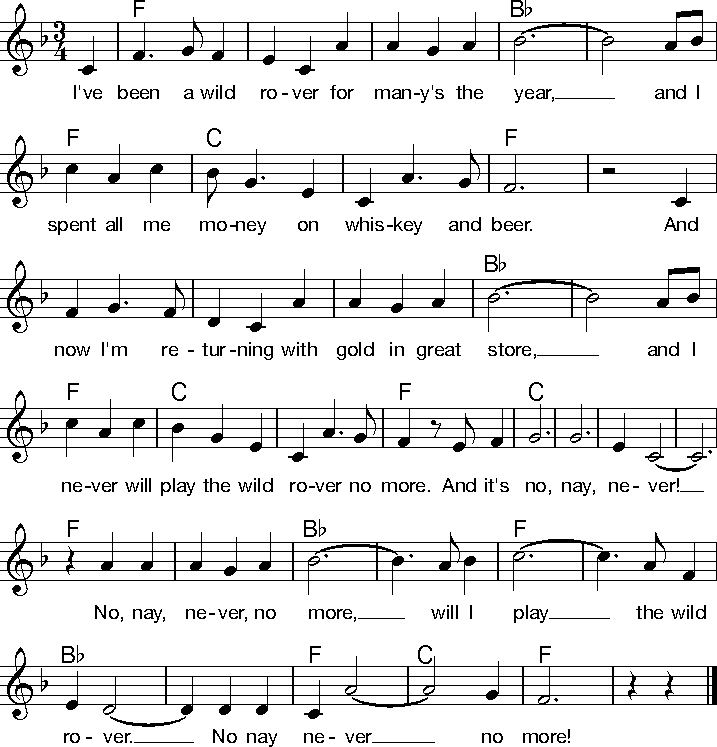
\includegraphics[draft=false, width=1\textwidth]{Noten/Lied083a.pdf}

\beginverse
I \[F]brought up from me pocket ten souvereigns \[Bb]bright
And the \[F]landlady's \[C]eyes opened wide with de\[F]light,
She said: 'I have whiskey and wines oh the \[Bb]best',
And the \[F]words that you've \[C]told me were only in \[F]jest.
\endverse

\beginchorus
And it's \[C]no, ney never,\[F] no, nay, never no \[Bb]more
I will \[F]play the wild \[Bb]rover, no \[F]never \[C]no \[F]more.
\endchorus

\beginverse
I'll go ^home to my parents, confess what I've ^done,
And I'll ^ask them to ^pardon their prodigal ^son.
And when they've caressed me, as oft' times be^fore,
I ^never will ^play the wild rover no ^more.
\endverse

\printchorus

\endsong

\beginscripture{}
The Wild Rover ist ein irisches Volkslied, dessen Quellen umstritten sind.
Tom Devine zufolge wurde das Lied als Abstinenzlerlied geschrieben. Es entstand nicht früher als 1829. Es erzählt die biblische Geschichte vom verlorenen Sohn auf irisch. Das Lied wurde im Buch „The American Songster“ gefunden, veröffentlicht in den USA von W.A. Leary im Jahr 1845, und gelangte durch die Abstinenzbewegung von Schottland nach Amerika. Eine andere in den USA gedruckte Version fand man im „Forget-Me-Not Songster“, veröffentlicht von Locke um 1850. Eine andere Entstehunggeschichte des Liedes basiert auf der Tatsache, dass eine Sammlung von Balladen, Entstehungzeit datiert zwischen 1813 und 1838, in der Bodleian Library steht. Der Veröffentlicher, Catnach, lebte im "7 Dials" Gebiet von Covent Garden, London. Der Band enthält "The Wild Rover". Die Greig-Duncan Sammlung enthält nicht weniger als sechs unterschiedliche Versionen des Liedes. Es wurde von Gavin Greig zusammengestellt.
\endscripture
